\chapter{\en{Virtual Environment Set up}}

\section{\en{GNS3 Installation}}

Το \en{GNS3} είναι ένα λογισμικό που χρησιμοποιείται για την εξομοίωση, τη διαμόρφωση και τη δοκιμή ενός περιβάλλοντος δικτύου. Είναι
είναι ένα ελεύθερο λογισμικό ανοικτού κώδικα και μπορείτε να το κατεβάσετε από τον επίσημο δικτυακό τόπο 
\en{https://www.gns3.com/} .

Το \en{GNS3} αποτελείται από δύο στοιχεία. Το ολοκληρωμένο λογισμικό (\en{GUI}) το οποίο είναι ένα γραφικό 
διεπαφή χρήστη και την εικονική μηχανή (\en{VM}), η οποία είναι ένας διακομιστής που εκτελείται σε εικονικό περιβάλλον και παρέχει καλύτερο μέγεθος τοπολογίας και υποστήριξη συσκευών.
Η εγκατάσταση είναι απλή και θα πρέπει να χρησιμοποιούνται οι προεπιλεγμένες επιλογές.

Για να γίνει σωστά η εγκατάσταση θα πρέπει το \en{software version} του \en{GNS3} να είναι το ίδιο με το
\en{software version} του \en{GNS3 VM}. Όταν λοιπόν γίνει η εγκατάσταση και ανοίγουμε το \en{GNS3 GUI}
αυτή η ενέργεια θα κάνει \en{trigger} το \en{booting} του \en{GNS3 VM}

Μόλις γίνει η εγκατάσταση μπορεί να ανοίξει η εφαρμογή και να κάνουμε \en{import cisco IOS images}. Στην παρακάτω
εικόνα μπορούμε να δούμε τι γίνεται όταν ανοίγουμε το \en{GNS3}. 

\begin{figure}[htb]
	\centering
	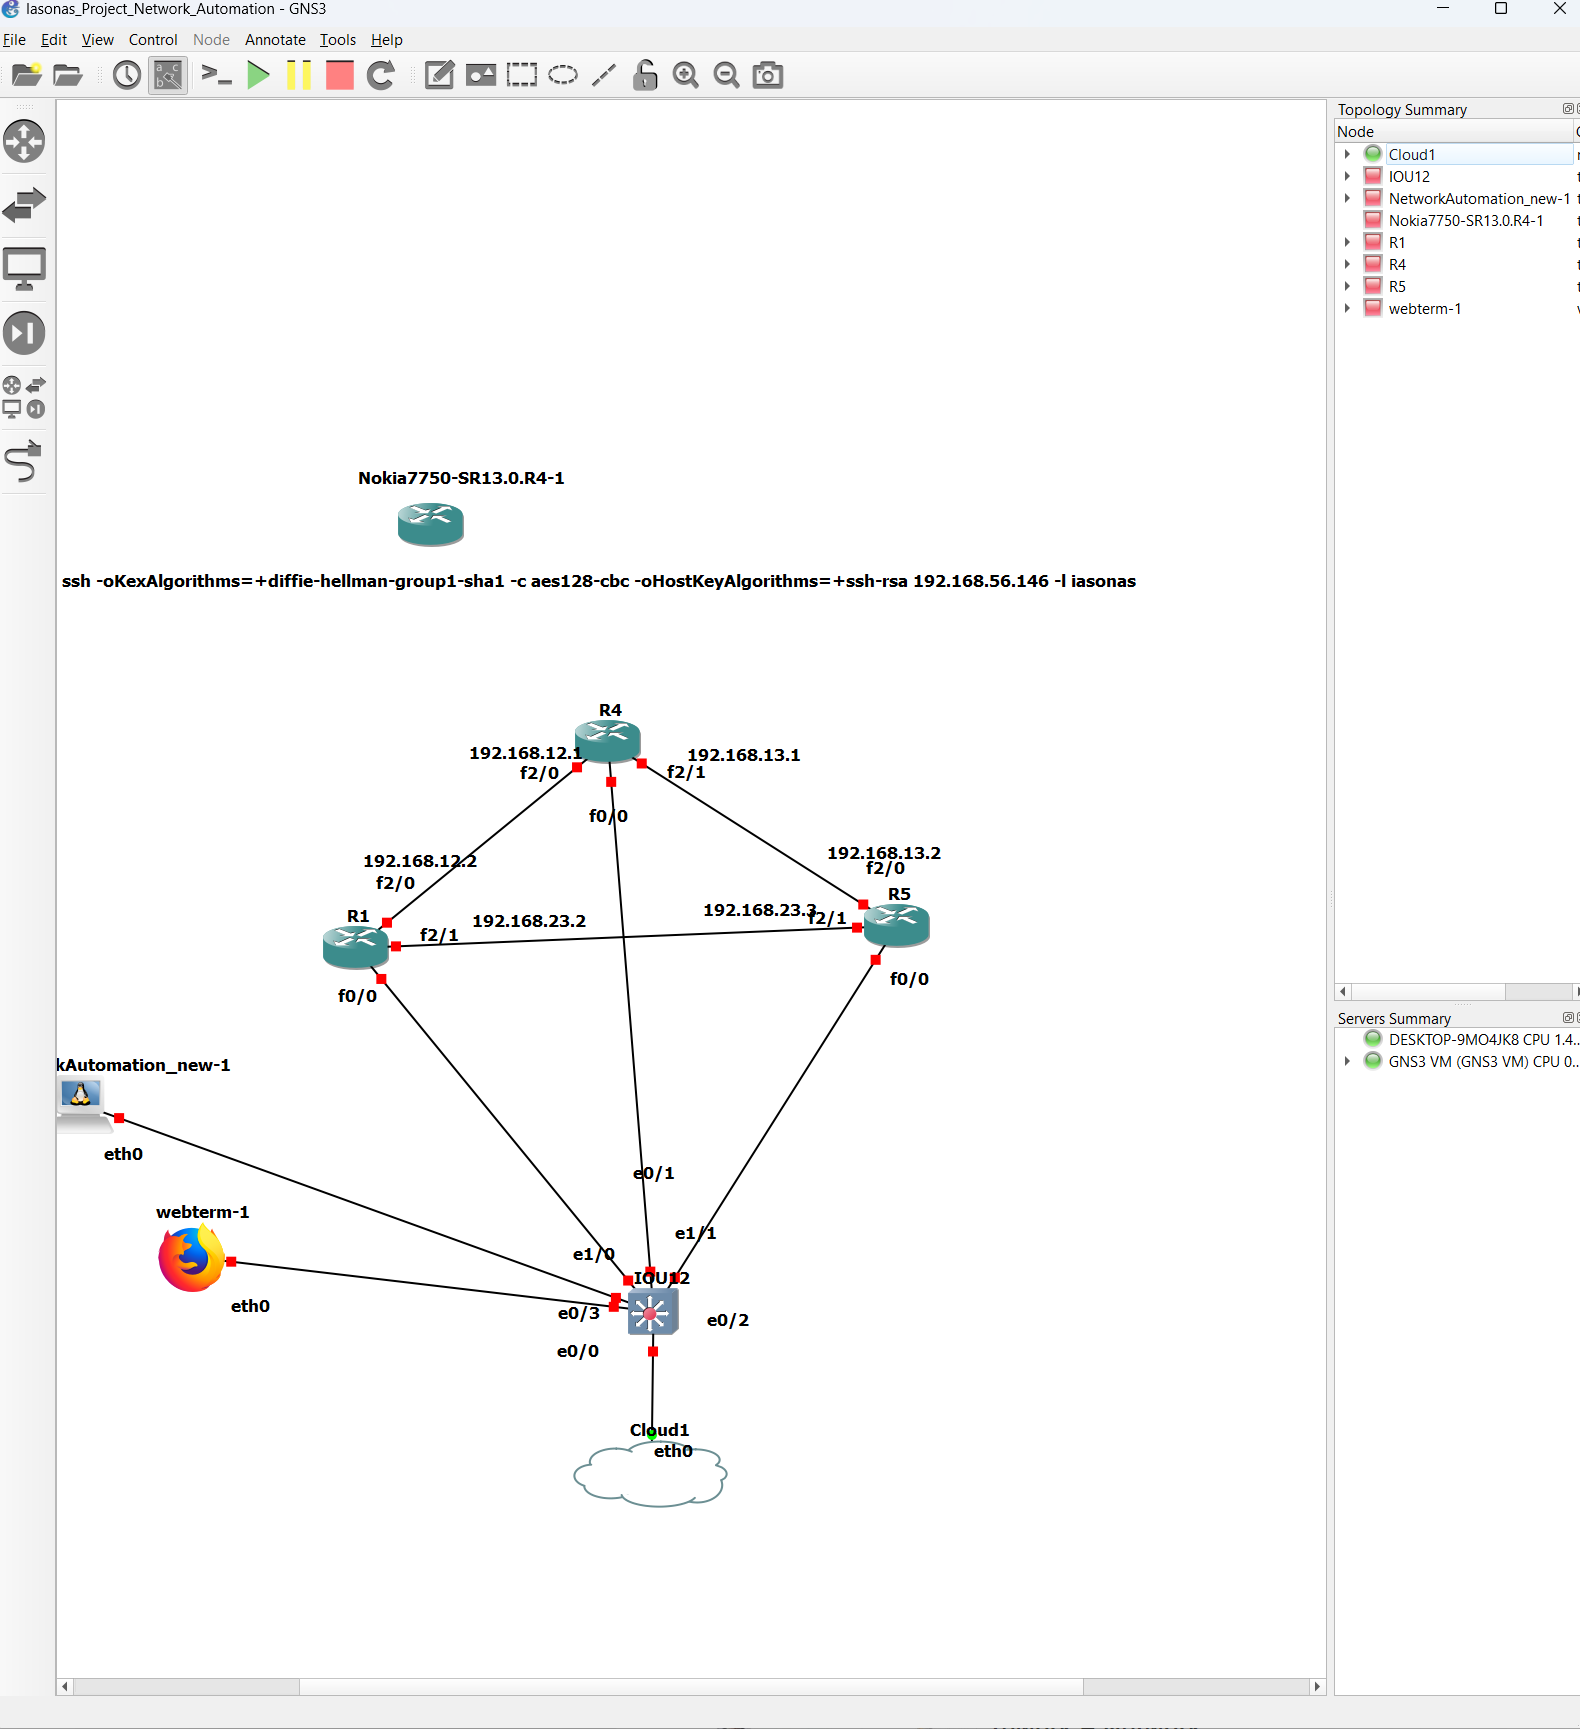
\includegraphics[width=0.7\textwidth]{graphics/gns3_homepage.png}
	\caption{\en{GNS3 homepage} }
\end{figure}

Προκειμένου να μπορέσει να επικοινωνήσει το \en{PC} μας στο τοπικό δίκτυο με το \en{GNS3 VM} στο τοπικό δίκτυο
θα πρέπει να γίνουν κάποιες ρυθμίσεις.